\section{Use-Case Analysis}

\subsection{Actor model}

PizzaHUST involves four human actor groups and one supporting external system. The actor model is derived from the original analysis artifacts and the maintained use-case documentation.

\begingroup
\small
\captionof{table}{Actor model for PizzaHUST}\label{tab:actor-model}
\begin{tabular}{L{0.20\linewidth} L{0.22\linewidth} L{0.49\linewidth}}
\toprule
\textbf{Actor} & \textbf{Type} & \textbf{Main interaction with the system} \\
\midrule
Guest & Primary external actor & Browses menus, views product details, customizes products, places COD orders, and tracks orders without creating an account. \\
Customer & Primary external actor & Inherits all guest behaviors and additionally uses authentication, profile management, loyalty functions, and personal order history. \\
Admin / Store Owner & Primary internal actor & Manages catalog data, combo campaigns, customers, orders, and reporting information. \\
Kitchen Staff & Primary internal actor & Receives queued orders, updates kitchen-side progress, and performs dispatch handoff actions. \\
Third-Party Delivery Service & Supporting external actor & Receives delivery-booking requests and pushes delivery-status updates back to PizzaHUST. \\
\bottomrule
\end{tabular}
\endgroup

The most important actor relationship is the generalization between \textbf{Guest} and \textbf{Customer}. A customer keeps all public ordering capabilities of a guest and gains account-specific capabilities such as profile, order history, and loyalty operations.

\subsection{Use-case overview}

Figure~\ref{fig:use-case-overview} presents the updated original use-case overview for PizzaHUST. This figure is treated as the authoritative analysis-level overview because it reflects the intended system scope before later implementation-specific refinements.

\begin{figure}[htbp]
    \centering
    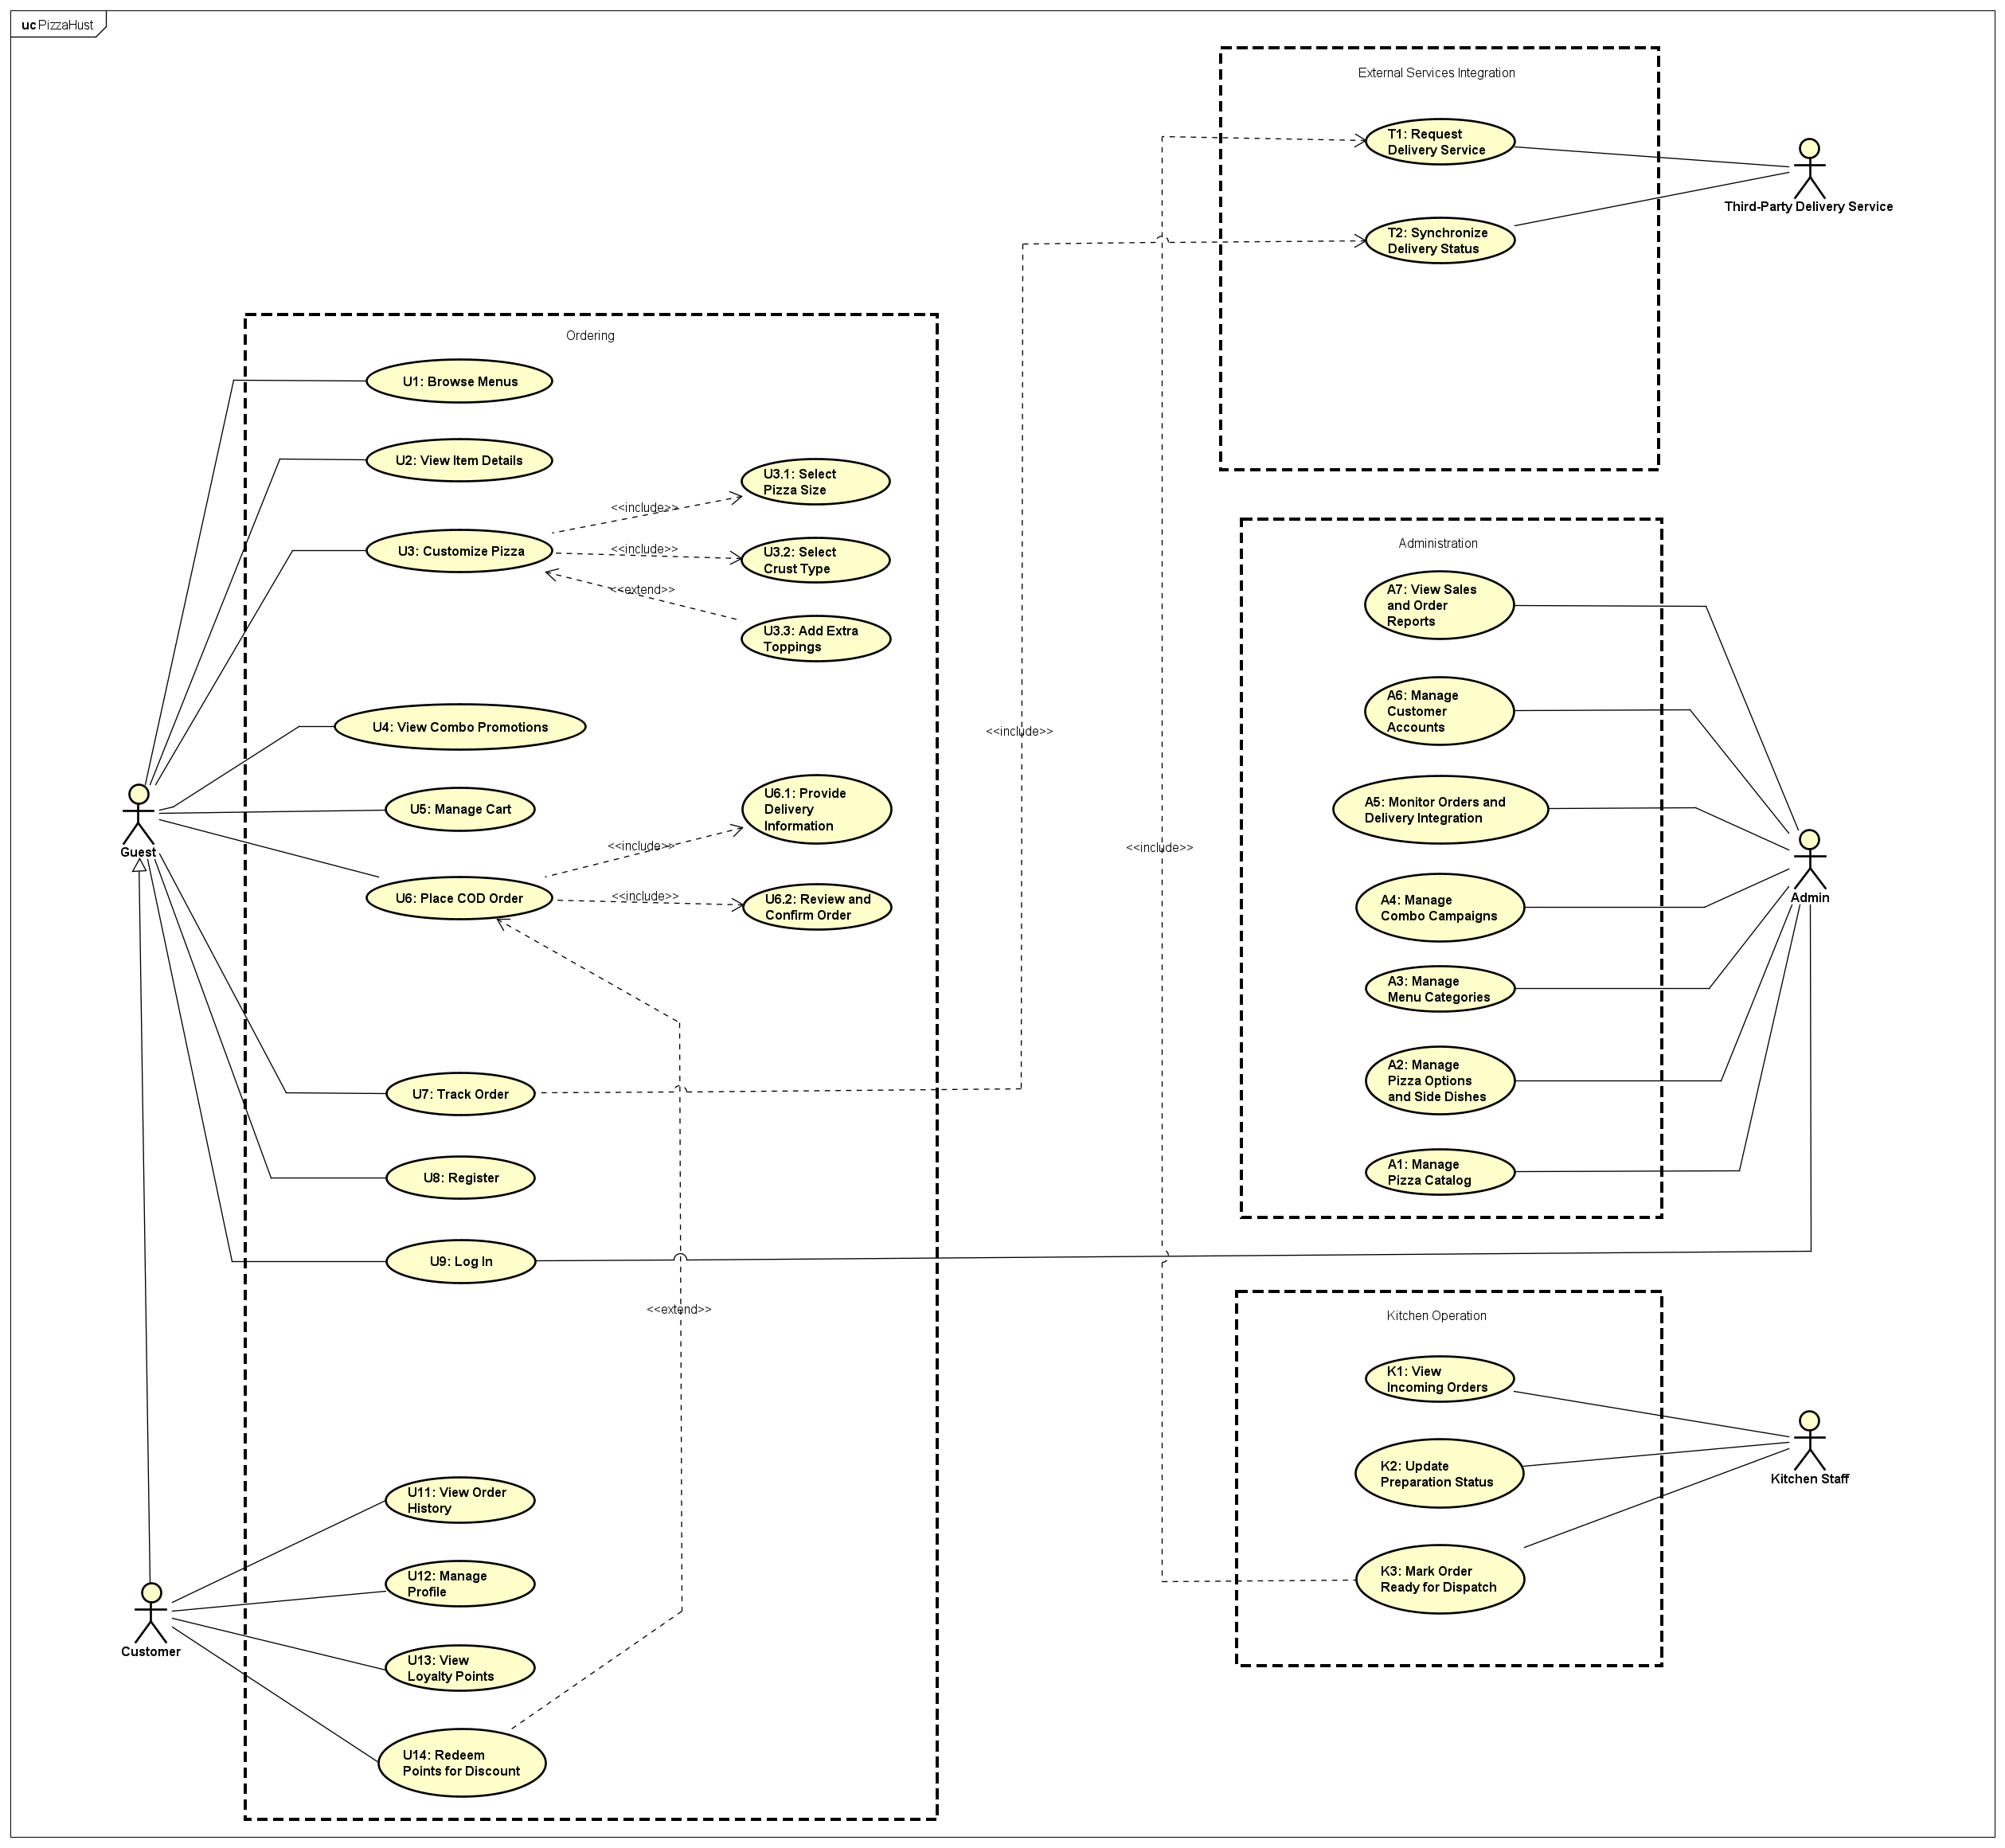
\includegraphics[width=\textwidth,height=0.86\textheight,keepaspectratio]{../PizzaHust.png}
    \caption{Overall use-case overview of PizzaHUST from the updated analysis artifact}
    \label{fig:use-case-overview}
\end{figure}

The overview shows four major interaction areas: customer ordering and account behavior, administrative management, kitchen operations, and delivery-service integration. These same areas later reappear in the architecture, database, API, and testing sections, which makes the use-case model the main bridge between requirements analysis and implementation evidence.

\subsection{Use-case relationships}

The use-case model is not a flat list of isolated actions. Several relationships are especially important:

\begin{itemize}
    \item \textbf{Actor generalization:} Customer extends Guest because authenticated users still perform the same public ordering actions.
    \item \textbf{Include relationships:} U6 \emph{Place COD Order} and U7 \emph{Track Order} depend on mandatory sub-behaviors such as delivery-information handling and delivery-state synchronization.
    \item \textbf{Extend relationships:} optional behaviors such as U14 \emph{Redeem Points for Discount} and U16 \emph{Add Order Notes} extend a base ordering flow rather than replacing it.
    \item \textbf{Operational interaction:} K3 \emph{Mark Order Ready for Dispatch} and A5 \emph{Monitor Orders and Delivery Exceptions} connect internal order handling with external delivery-service behavior T1 and T2.
\end{itemize}

\subsection{Detailed use case analysis}

This subsection presents the designed use-case set through a single consistent specification format. For readability, every use case is written as a bordered two-column table with the same fields: use-case code, use-case name, actor(s), brief description, preconditions, postconditions, basic flow of events, alternative flows of events, input data, and output data.

\setlength{\LTleft}{0pt}
\setlength{\LTright}{0pt}
\renewcommand{\arraystretch}{1.08}

\newcommand{\ucfield}[2]{\textbf{#1} & #2 \\ \hline}

\subsubsection*{Customer-facing use cases}

\begingroup
\footnotesize
\begin{longtable}{|>{\raggedright\arraybackslash}p{0.24\linewidth}|>{\raggedright\arraybackslash}p{0.70\linewidth}|}
\caption{Detailed use-case specification for U1: Browse Menus}\label{tab:uc-u1}\\ \hline
\textbf{Field} & \textbf{Description} \\ \hline
\endfirsthead
\caption[]{Detailed use-case specification for U1: Browse Menus (continued)}\\ \hline
\textbf{Field} & \textbf{Description} \\ \hline
\endhead
\ucfield{Use Case Code}{U1}
\ucfield{Use Case Name}{Browse Menus}
\ucfield{Actor(s)}{Guest, Customer}
\ucfield{Brief Description}{The user views active menu categories and products in order to find dishes available for ordering.}
\ucfield{Preconditions}{The system contains at least one active category and one active dish.}
\ucfield{Postconditions}{None. This is a read-only use case that may lead to U2 or U4.}
\ucfield{Basic Flow of Events}{1. The user opens the menu page. \newline 2. The system retrieves active categories and dishes. \newline 3. The system displays category filters and dish cards. \newline 4. The user changes the category filter. \newline 5. The system refreshes the visible menu list.}
\ucfield{Alternative Flows of Events}{1. If the selected category has no active dishes, the system shows an empty-category message. \newline 2. If the catalog request fails, the system shows an error state and a retry control.}
\ucfield{Input Data}{Optional category filter selected by the user.}
\ucfield{Output Data}{Active categories and visible dish cards.}
\end{longtable}
\endgroup

\begingroup
\footnotesize
\begin{longtable}{|>{\raggedright\arraybackslash}p{0.24\linewidth}|>{\raggedright\arraybackslash}p{0.70\linewidth}|}
\caption{Detailed use-case specification for U2: View Item Details}\label{tab:uc-u2}\\ \hline
\textbf{Field} & \textbf{Description} \\ \hline
\endfirsthead
\caption[]{Detailed use-case specification for U2: View Item Details (continued)}\\ \hline
\textbf{Field} & \textbf{Description} \\ \hline
\endhead
\ucfield{Use Case Code}{U2}
\ucfield{Use Case Name}{View Item Details}
\ucfield{Actor(s)}{Guest, Customer}
\ucfield{Brief Description}{The user opens a dish detail page to inspect product information and available customization options before ordering.}
\ucfield{Preconditions}{The selected dish exists and is active.}
\ucfield{Postconditions}{None. This is a read-only use case that may lead to U3 or U5.}
\ucfield{Basic Flow of Events}{1. The user selects a dish from the menu. \newline 2. The system retrieves the dish detail and enabled option groups. \newline 3. The system displays the dish name, image, base price, and customization entry point. \newline 4. The user reviews the information and decides whether to customize or add the item to the cart.}
\ucfield{Alternative Flows of Events}{1. If the dish becomes inactive after the menu page loads, the system reports that the item is no longer available. \newline 2. If the item is a simple side dish, the system hides pizza-specific customization controls.}
\ucfield{Input Data}{Selected dish identifier.}
\ucfield{Output Data}{Detailed item information and enabled option groups.}
\end{longtable}
\endgroup

\begingroup
\footnotesize
\begin{longtable}{|>{\raggedright\arraybackslash}p{0.24\linewidth}|>{\raggedright\arraybackslash}p{0.70\linewidth}|}
\caption{Detailed use-case specification for U3: Customize Pizza}\label{tab:uc-u3}\\ \hline
\textbf{Field} & \textbf{Description} \\ \hline
\endfirsthead
\caption[]{Detailed use-case specification for U3: Customize Pizza (continued)}\\ \hline
\textbf{Field} & \textbf{Description} \\ \hline
\endhead
\ucfield{Use Case Code}{U3}
\ucfield{Use Case Name}{Customize Pizza}
\ucfield{Actor(s)}{Guest, Customer}
\ucfield{Brief Description}{The user configures a pizza by selecting required and optional options, then obtains a server-validated quote before adding the line to the cart.}
\ucfield{Preconditions}{The target pizza is active and exposes the required option groups for customization.}
\ucfield{Postconditions}{A valid configured pizza line is ready to be added to the cart; no order is created yet.}
\ucfield{Basic Flow of Events}{1. The user opens the pizza customizer from the item detail page. \newline 2. The system shows enabled option groups such as size, crust, and toppings. \newline 3. The user selects required and optional options. \newline 4. The system sends the configuration to the quoting endpoint and returns the authoritative line total. \newline 5. The user confirms the configuration and proceeds to cart storage.}
\ucfield{Alternative Flows of Events}{1. If a selected option is no longer enabled, the system rejects the quote and asks the user to reselect. \newline 2. If a required group has no selection, the system blocks add-to-cart. \newline 3. If the dish becomes inactive during customization, the flow ends with an availability error.}
\ucfield{Input Data}{Selected option identifiers, optional dish note, and quantity.}
\ucfield{Output Data}{Server-computed line total and normalized selected-option summary.}
\end{longtable}
\endgroup

\begingroup
\footnotesize
\begin{longtable}{|>{\raggedright\arraybackslash}p{0.24\linewidth}|>{\raggedright\arraybackslash}p{0.70\linewidth}|}
\caption{Detailed use-case specification for U4: View Combo Promotions}\label{tab:uc-u4}\\ \hline
\textbf{Field} & \textbf{Description} \\ \hline
\endfirsthead
\caption[]{Detailed use-case specification for U4: View Combo Promotions (continued)}\\ \hline
\textbf{Field} & \textbf{Description} \\ \hline
\endhead
\ucfield{Use Case Code}{U4}
\ucfield{Use Case Name}{View Combo Promotions}
\ucfield{Actor(s)}{Guest, Customer}
\ucfield{Brief Description}{The user views active combo campaigns, including components, bundle pricing, and calculated savings.}
\ucfield{Preconditions}{At least one combo is active in the current validity window.}
\ucfield{Postconditions}{None. This is a read-only use case that may lead to U15.}
\ucfield{Basic Flow of Events}{1. The user opens the combo promotions page. \newline 2. The system retrieves currently active combos. \newline 3. The system displays each combo with name, components, price, and savings. \newline 4. The user opens a combo to inspect its details and possible customization path.}
\ucfield{Alternative Flows of Events}{1. If no combos are active, the system shows an empty state. \newline 2. If a combo is over-priced relative to its parts, the system still shows it but displays zero savings. \newline 3. If a combo expires while being viewed, the system blocks further ordering actions.}
\ucfield{Input Data}{Optional combo selected for detail viewing.}
\ucfield{Output Data}{Active combo list and combo detail information.}
\end{longtable}
\endgroup

\begingroup
\footnotesize
\begin{longtable}{|>{\raggedright\arraybackslash}p{0.24\linewidth}|>{\raggedright\arraybackslash}p{0.70\linewidth}|}
\caption{Detailed use-case specification for U5: Manage Cart}\label{tab:uc-u5}\\ \hline
\textbf{Field} & \textbf{Description} \\ \hline
\endfirsthead
\caption[]{Detailed use-case specification for U5: Manage Cart (continued)}\\ \hline
\textbf{Field} & \textbf{Description} \\ \hline
\endhead
\ucfield{Use Case Code}{U5}
\ucfield{Use Case Name}{Manage Cart}
\ucfield{Actor(s)}{Guest, Customer}
\ucfield{Brief Description}{The user reviews, edits, re-quotes, and removes intended order lines before proceeding to checkout.}
\ucfield{Preconditions}{A cart exists for the current guest session or authenticated customer session.}
\ucfield{Postconditions}{The cart reflects the latest valid user selections and authoritative pricing; no order is created yet.}
\ucfield{Basic Flow of Events}{1. The user opens the cart page. \newline 2. The system displays all cart lines with options, quantities, and line totals. \newline 3. The user edits quantity, configuration, or removes a line. \newline 4. The system re-quotes the cart and refreshes subtotal and discounts. \newline 5. The user proceeds to checkout.}
\ucfield{Alternative Flows of Events}{1. If a line's dish or combo becomes unavailable, the system flags that line for correction or removal. \newline 2. If a line contains an option no longer enabled for the dish, the system forces re-customization. \newline 3. If the cart is empty, checkout remains unavailable.}
\ucfield{Input Data}{Cart-line identifier, new quantity, or revised configuration.}
\ucfield{Output Data}{Updated line totals, subtotal, and combo-discount values.}
\end{longtable}
\endgroup

\begingroup
\footnotesize
\begin{longtable}{|>{\raggedright\arraybackslash}p{0.24\linewidth}|>{\raggedright\arraybackslash}p{0.70\linewidth}|}
\caption{Detailed use-case specification for U6: Place COD Order}\label{tab:uc-u6}\\ \hline
\textbf{Field} & \textbf{Description} \\ \hline
\endfirsthead
\caption[]{Detailed use-case specification for U6: Place COD Order (continued)}\\ \hline
\textbf{Field} & \textbf{Description} \\ \hline
\endhead
\ucfield{Use Case Code}{U6}
\ucfield{Use Case Name}{Place COD Order}
\ucfield{Actor(s)}{Guest, Customer}
\ucfield{Brief Description}{The user submits the cart as a cash-on-delivery order after delivery validation and final server-side order checking.}
\ucfield{Preconditions}{The cart contains at least one valid line; if loyalty redemption is used, the actor is an authenticated customer.}
\ucfield{Postconditions}{A new order is created with an order code and initial processing state; the order enters kitchen processing.}
\ucfield{Basic Flow of Events}{1. The user proceeds from the cart to checkout. \newline 2. The system displays the recipient and delivery form. \newline 3. The user enters recipient information, phone number, address, and optional delivery note. \newline 4. The system validates the address, applies the fixed delivery fee, and recalculates totals. \newline 5. The customer may optionally redeem loyalty points. \newline 6. The user confirms the COD purchase. \newline 7. The system revalidates all lines and persists the order with a generated code. \newline 8. The system shows the confirmation page and tracking entry point.}
\ucfield{Alternative Flows of Events}{1. If the address is outside the supported service area, the system rejects the address and blocks submission. \newline 2. If the phone number format is invalid, the system highlights the error. \newline 3. If a cart line becomes unavailable during final validation, the system returns the user to cart correction. \newline 4. If loyalty redemption exceeds the balance or cap, the system rejects that redemption.}
\ucfield{Input Data}{Recipient name, phone number, delivery address, optional delivery note, and optional redeemed points.}
\ucfield{Output Data}{Order code, persisted order summary, delivery fee, loyalty discount if any, and final COD total.}
\end{longtable}
\endgroup

\begingroup
\footnotesize
\begin{longtable}{|>{\raggedright\arraybackslash}p{0.24\linewidth}|>{\raggedright\arraybackslash}p{0.70\linewidth}|}
\caption{Detailed use-case specification for U7: Track Order}\label{tab:uc-u7}\\ \hline
\textbf{Field} & \textbf{Description} \\ \hline
\endfirsthead
\caption[]{Detailed use-case specification for U7: Track Order (continued)}\\ \hline
\textbf{Field} & \textbf{Description} \\ \hline
\endhead
\ucfield{Use Case Code}{U7}
\ucfield{Use Case Name}{Track Order}
\ucfield{Actor(s)}{Guest, Customer}
\ucfield{Brief Description}{The user follows order progress through a tracking view that exposes minimal public information for guests and richer detail for the owning customer.}
\ucfield{Preconditions}{The target order exists; guest tracking requires a valid order code.}
\ucfield{Postconditions}{None. This is a read-only use case.}
\ucfield{Basic Flow of Events}{1. The user opens the tracking page and provides the order code, or follows a direct tracking link. \newline 2. The system resolves the order and returns the visible tracking projection. \newline 3. The system displays the status timeline and promised delivery time. \newline 4. The tracking view continues polling for updates as the order progresses.}
\ucfield{Alternative Flows of Events}{1. If the order code is unknown, the system shows an order-not-found message. \newline 2. If lookup rate limits are exceeded, the system blocks further requests temporarily. \newline 3. If the order becomes cancelled or delivery-failed, the system shows the terminal state and ends tracking progression.}
\ucfield{Input Data}{Order code for guest lookup, or authenticated customer session for owned orders.}
\ucfield{Output Data}{Current status, status timeline, promised time, and privacy-filtered recipient information.}
\end{longtable}
\endgroup

\begingroup
\footnotesize
\begin{longtable}{|>{\raggedright\arraybackslash}p{0.24\linewidth}|>{\raggedright\arraybackslash}p{0.70\linewidth}|}
\caption{Detailed use-case specification for U8: Register Account}\label{tab:uc-u8}\\ \hline
\textbf{Field} & \textbf{Description} \\ \hline
\endfirsthead
\caption[]{Detailed use-case specification for U8: Register Account (continued)}\\ \hline
\textbf{Field} & \textbf{Description} \\ \hline
\endhead
\ucfield{Use Case Code}{U8}
\ucfield{Use Case Name}{Register Account}
\ucfield{Actor(s)}{Guest}
\ucfield{Brief Description}{A guest creates a customer account by submitting personal identification and login credentials.}
\ucfield{Preconditions}{The visitor is not currently authenticated.}
\ucfield{Postconditions}{A customer account exists and an authenticated session is started.}
\ucfield{Basic Flow of Events}{1. The guest opens the registration page. \newline 2. The system displays the registration form. \newline 3. The guest enters full name, phone number, password, and address. \newline 4. The system validates uniqueness and password rules. \newline 5. The system creates the account, starts the session, and redirects the user back into the storefront.}
\ucfield{Alternative Flows of Events}{1. If the phone number is already registered, the system rejects the registration. \newline 2. If the password does not satisfy the strength policy, the system highlights the rule violation. \newline 3. If registration rate limits are exceeded, the system temporarily rejects the request.}
\ucfield{Input Data}{Full name, phone number, password, and default address.}
\ucfield{Output Data}{Authenticated session and newly created customer profile.}
\end{longtable}
\endgroup

\begingroup
\footnotesize
\begin{longtable}{|>{\raggedright\arraybackslash}p{0.24\linewidth}|>{\raggedright\arraybackslash}p{0.70\linewidth}|}
\caption{Detailed use-case specification for U9: Log In}\label{tab:uc-u9}\\ \hline
\textbf{Field} & \textbf{Description} \\ \hline
\endfirsthead
\caption[]{Detailed use-case specification for U9: Log In (continued)}\\ \hline
\textbf{Field} & \textbf{Description} \\ \hline
\endhead
\ucfield{Use Case Code}{U9}
\ucfield{Use Case Name}{Log In}
\ucfield{Actor(s)}{Customer}
\ucfield{Brief Description}{A registered customer authenticates with phone number and password to access account-protected features.}
\ucfield{Preconditions}{The customer account exists and is not locked.}
\ucfield{Postconditions}{The customer is authenticated and can access account-based use cases.}
\ucfield{Basic Flow of Events}{1. The customer opens the login page and enters phone number and password. \newline 2. The system verifies the credentials against the stored password hash. \newline 3. The system starts an authenticated session and issues the CSRF protection token. \newline 4. The system merges any guest-session cart into the account cart and redirects the customer.}
\ucfield{Alternative Flows of Events}{1. If the credentials are invalid, the system shows a generic authentication error. \newline 2. If the account is locked by an administrator, the system refuses login. \newline 3. If login rate limits are exceeded, the system temporarily rejects the request.}
\ucfield{Input Data}{Registered phone number and password.}
\ucfield{Output Data}{Authenticated customer session and merged cart context if applicable.}
\end{longtable}
\endgroup

\begingroup
\footnotesize
\begin{longtable}{|>{\raggedright\arraybackslash}p{0.24\linewidth}|>{\raggedright\arraybackslash}p{0.70\linewidth}|}
\caption{Detailed use-case specification for U11: View Order History}\label{tab:uc-u11}\\ \hline
\textbf{Field} & \textbf{Description} \\ \hline
\endfirsthead
\caption[]{Detailed use-case specification for U11: View Order History (continued)}\\ \hline
\textbf{Field} & \textbf{Description} \\ \hline
\endhead
\ucfield{Use Case Code}{U11}
\ucfield{Use Case Name}{View Order History}
\ucfield{Actor(s)}{Customer}
\ucfield{Brief Description}{An authenticated customer views previous and current orders associated with their own account.}
\ucfield{Preconditions}{The customer is logged in.}
\ucfield{Postconditions}{None. This is a read-only use case that may lead to U7 for in-progress orders.}
\ucfield{Basic Flow of Events}{1. The customer opens the order history page. \newline 2. The system lists the customer's orders, newest first. \newline 3. The customer selects one order. \newline 4. The system shows complete order details, including lines, totals, and status timeline. \newline 5. The customer may jump to live tracking for an in-progress order.}
\ucfield{Alternative Flows of Events}{1. If the account has no orders, the system shows an empty state linking back to ordering. \newline 2. If the customer attempts to access an order belonging to another account, the system denies access.}
\ucfield{Input Data}{Customer session and selected order identifier.}
\ucfield{Output Data}{Paginated order list and full detail for the selected order.}
\end{longtable}
\endgroup

\begingroup
\footnotesize
\begin{longtable}{|>{\raggedright\arraybackslash}p{0.24\linewidth}|>{\raggedright\arraybackslash}p{0.70\linewidth}|}
\caption{Detailed use-case specification for U12: Manage Profile}\label{tab:uc-u12}\\ \hline
\textbf{Field} & \textbf{Description} \\ \hline
\endfirsthead
\caption[]{Detailed use-case specification for U12: Manage Profile (continued)}\\ \hline
\textbf{Field} & \textbf{Description} \\ \hline
\endhead
\ucfield{Use Case Code}{U12}
\ucfield{Use Case Name}{Manage Profile}
\ucfield{Actor(s)}{Customer}
\ucfield{Brief Description}{An authenticated customer edits profile information such as full name, default address, avatar, and password.}
\ucfield{Preconditions}{The customer is logged in.}
\ucfield{Postconditions}{The edited profile values are persisted; any supported credential change takes effect for later sessions.}
\ucfield{Basic Flow of Events}{1. The customer opens the profile page. \newline 2. The system displays current profile data with phone number treated as read-only. \newline 3. The customer edits supported profile fields and submits the form. \newline 4. The system validates and persists the changes. \newline 5. The customer may also upload an avatar or change password from the same account surface.}
\ucfield{Alternative Flows of Events}{1. If a field fails validation, the system rejects the update and highlights the problem. \newline 2. If an avatar upload fails type or size validation, the system rejects that file. \newline 3. If the current password is wrong during a password-change attempt, the system rejects the credential change.}
\ucfield{Input Data}{Edited profile fields, and in full scope optional avatar file or password-change data.}
\ucfield{Output Data}{Updated profile summary and confirmation feedback.}
\end{longtable}
\endgroup

\begingroup
\footnotesize
\begin{longtable}{|>{\raggedright\arraybackslash}p{0.24\linewidth}|>{\raggedright\arraybackslash}p{0.70\linewidth}|}
\caption{Detailed use-case specification for U13: View Loyalty Points}\label{tab:uc-u13}\\ \hline
\textbf{Field} & \textbf{Description} \\ \hline
\endfirsthead
\caption[]{Detailed use-case specification for U13: View Loyalty Points (continued)}\\ \hline
\textbf{Field} & \textbf{Description} \\ \hline
\endhead
\ucfield{Use Case Code}{U13}
\ucfield{Use Case Name}{View Loyalty Points}
\ucfield{Actor(s)}{Customer}
\ucfield{Brief Description}{An authenticated customer checks the current loyalty balance and the rules for earning and spending points.}
\ucfield{Preconditions}{The customer is logged in.}
\ucfield{Postconditions}{None. This is a read-only use case.}
\ucfield{Basic Flow of Events}{1. The customer opens the loyalty page or inspects the balance shown in the authenticated header. \newline 2. The system displays the current balance and the earning and redemption rules. \newline 3. The system shows the loyalty history for recent earn and redemption activity.}
\ucfield{Alternative Flows of Events}{If the balance is zero and there is no loyalty history, the system shows an explanatory empty state.}
\ucfield{Input Data}{Authenticated customer identity.}
\ucfield{Output Data}{Current loyalty balance, rule explanation, and loyalty history entries.}
\end{longtable}
\endgroup

\begingroup
\footnotesize
\begin{longtable}{|>{\raggedright\arraybackslash}p{0.24\linewidth}|>{\raggedright\arraybackslash}p{0.70\linewidth}|}
\caption{Detailed use-case specification for U14: Redeem Points for Discount}\label{tab:uc-u14}\\ \hline
\textbf{Field} & \textbf{Description} \\ \hline
\endfirsthead
\caption[]{Detailed use-case specification for U14: Redeem Points for Discount (continued)}\\ \hline
\textbf{Field} & \textbf{Description} \\ \hline
\endhead
\ucfield{Use Case Code}{U14}
\ucfield{Use Case Name}{Redeem Points for Discount}
\ucfield{Actor(s)}{Customer}
\ucfield{Brief Description}{During checkout, the customer converts loyalty points into a discount on the current order, subject to balance and percentage-cap rules.}
\ucfield{Preconditions}{The customer is logged in, has a positive balance, and already has a valid quoted cart in checkout.}
\ucfield{Postconditions}{A valid loyalty discount is applied to the current order quote, and the corresponding points are reserved when the order is created.}
\ucfield{Basic Flow of Events}{1. The customer opens the redemption control during checkout. \newline 2. The customer enters the number of points to redeem. \newline 3. The system verifies that the requested points do not exceed the balance and discount cap. \newline 4. The system recalculates the order quote with the loyalty discount applied. \newline 5. The customer continues the checkout flow.}
\ucfield{Alternative Flows of Events}{1. If the requested points exceed the available balance, the system rejects the request. \newline 2. If the requested discount exceeds the allowed percentage of the subtotal, the system rejects the request with a validation error. \newline 3. If the order is later cancelled or delivery fails, the reserved points are released back to the customer.}
\ucfield{Input Data}{Number of points to redeem.}
\ucfield{Output Data}{Applied loyalty discount, recalculated order total, and visible remaining balance.}
\end{longtable}
\endgroup

\begingroup
\footnotesize
\begin{longtable}{|>{\raggedright\arraybackslash}p{0.24\linewidth}|>{\raggedright\arraybackslash}p{0.70\linewidth}|}
\caption{Detailed use-case specification for U15: Customize Combo}\label{tab:uc-u15}\\ \hline
\textbf{Field} & \textbf{Description} \\ \hline
\endfirsthead
\caption[]{Detailed use-case specification for U15: Customize Combo (continued)}\\ \hline
\textbf{Field} & \textbf{Description} \\ \hline
\endhead
\ucfield{Use Case Code}{U15}
\ucfield{Use Case Name}{Customize Combo}
\ucfield{Actor(s)}{Guest, Customer}
\ucfield{Brief Description}{The user resolves combo choice slots into concrete products and configures any pizza items inside the combo before the system produces a final quoted combo line.}
\ucfield{Preconditions}{The combo is currently active and each choice slot has at least one eligible product.}
\ucfield{Postconditions}{A resolved combo line with authoritative pricing is ready for cart storage; no order is created yet.}
\ucfield{Basic Flow of Events}{1. The user opens the combo customizer from the combo detail page. \newline 2. The system displays fixed components and customer-choice slots, including surcharge information. \newline 3. The user resolves each slot by choosing concrete products. \newline 4. The user configures pizza-specific options inside the chosen products where needed. \newline 5. The system quotes the fully resolved combo line and shows the resulting charged total and savings. \newline 6. The user confirms the configuration.}
\ucfield{Alternative Flows of Events}{1. If a slot remains unresolved, the system blocks continuation. \newline 2. If the number of selected slot picks does not match the required quantity, the system asks for correction. \newline 3. If a picked product is invalid for the slot category or option rules fail, the system rejects the quote. \newline 4. If the combo leaves its active validity window, the system stops the ordering flow.}
\ucfield{Input Data}{Selected products for each slot, option selections for configurable items, optional dish notes, and quantity.}
\ucfield{Output Data}{Charged combo total, calculated savings, and a normalized resolved configuration summary.}
\end{longtable}
\endgroup

\begingroup
\footnotesize
\begin{longtable}{|>{\raggedright\arraybackslash}p{0.24\linewidth}|>{\raggedright\arraybackslash}p{0.70\linewidth}|}
\caption{Detailed use-case specification for U16: Add Order Notes}\label{tab:uc-u16}\\ \hline
\textbf{Field} & \textbf{Description} \\ \hline
\endfirsthead
\caption[]{Detailed use-case specification for U16: Add Order Notes (continued)}\\ \hline
\textbf{Field} & \textbf{Description} \\ \hline
\endhead
\ucfield{Use Case Code}{U16}
\ucfield{Use Case Name}{Add Order Notes}
\ucfield{Actor(s)}{Guest, Customer}
\ucfield{Brief Description}{The user adds free-text notes either for kitchen-side dish preparation or for courier-side delivery instructions.}
\ucfield{Preconditions}{The user is customizing a dish or combo line, or is filling the checkout delivery form.}
\ucfield{Postconditions}{Notes are stored in the appropriate audience-specific place: dish-level note or order-level delivery note.}
\ucfield{Basic Flow of Events}{1. The user writes an optional dish note during product customization. \newline 2. The system stores the note with that line and later shows it in cart and kitchen views. \newline 3. The user writes an optional delivery note during checkout. \newline 4. The system stores the delivery note with the order and reveals it only at the appropriate dispatch and tracking stages.}
\ucfield{Alternative Flows of Events}{1. If a note exceeds the length limit, the system truncates or rejects the excess input. \newline 2. If no notes are provided, the relevant note sections are simply omitted from later views.}
\ucfield{Input Data}{Free-text dish note and/or free-text delivery note.}
\ucfield{Output Data}{Persisted kitchen-facing note and courier-facing note associated with the correct entity.}
\end{longtable}
\endgroup

\subsubsection*{Administrative use cases}

\begingroup
\footnotesize
\begin{longtable}{|>{\raggedright\arraybackslash}p{0.24\linewidth}|>{\raggedright\arraybackslash}p{0.70\linewidth}|}
\caption{Detailed use-case specification for A1: Manage Pizza Catalog}\label{tab:uc-a1}\\ \hline
\textbf{Field} & \textbf{Description} \\ \hline
\endfirsthead
\caption[]{Detailed use-case specification for A1: Manage Pizza Catalog (continued)}\\ \hline
\textbf{Field} & \textbf{Description} \\ \hline
\endhead
\ucfield{Use Case Code}{A1}
\ucfield{Use Case Name}{Manage Pizza Catalog}
\ucfield{Actor(s)}{Admin / Store Owner}
\ucfield{Brief Description}{The administrator creates, edits, activates, deactivates, and imports pizza and side-dish records so the storefront reflects actual offerings.}
\ucfield{Preconditions}{The administrator is authenticated and target categories exist.}
\ucfield{Postconditions}{Catalog records are persisted and storefront visibility reflects the active state of each dish.}
\ucfield{Basic Flow of Events}{1. The administrator opens the catalog-management interface. \newline 2. The system lists existing dishes with key attributes and filters. \newline 3. The administrator creates a new dish or edits an existing one. \newline 4. The system displays the dish form and accepts the submitted values. \newline 5. The system validates and persists the dish. \newline 6. The administrator may optionally upload an image or perform CSV import operations.}
\ucfield{Alternative Flows of Events}{1. If the selected category is missing or inactive, the system rejects the save. \newline 2. If the uploaded image violates type or size rules, the system rejects the upload. \newline 3. If deactivation would break an active combo dependency, the system blocks that change until the combo is corrected.}
\ucfield{Input Data}{Dish name, kind, category, base price, active state, and optional image or CSV rows.}
\ucfield{Output Data}{Saved catalog entry, optional image URL, and optional import report.}
\end{longtable}
\endgroup

\begingroup
\footnotesize
\begin{longtable}{|>{\raggedright\arraybackslash}p{0.24\linewidth}|>{\raggedright\arraybackslash}p{0.70\linewidth}|}
\caption{Detailed use-case specification for A2: Manage Pizza Options and Side Dishes}\label{tab:uc-a2}\\ \hline
\textbf{Field} & \textbf{Description} \\ \hline
\endfirsthead
\caption[]{Detailed use-case specification for A2: Manage Pizza Options and Side Dishes (continued)}\\ \hline
\textbf{Field} & \textbf{Description} \\ \hline
\endhead
\ucfield{Use Case Code}{A2}
\ucfield{Use Case Name}{Manage Pizza Options and Side Dishes}
\ucfield{Actor(s)}{Admin / Store Owner}
\ucfield{Brief Description}{In the original analysis scope, the administrator managed pizza-option definitions and side-dish data through a dedicated use case. In the refined design, these responsibilities are absorbed by A1 and later option-management refinements.}
\ucfield{Preconditions}{The administrator is authenticated.}
\ucfield{Postconditions}{Option and side-dish data remain consistent with current catalog rules, even though the responsibility is distributed across refined administrative modules.}
\ucfield{Basic Flow of Events}{1. The administrator enters option or side-dish management. \newline 2. The system exposes the relevant editing surface. \newline 3. The administrator adds, edits, activates, or deactivates the target records. \newline 4. The system validates the changes and persists them so they affect ordering behavior.}
\ucfield{Alternative Flows of Events}{1. If an option configuration is invalid, the system rejects the update. \newline 2. If a side dish references invalid category data or conflicting values, the system blocks the save.}
\ucfield{Input Data}{Option definitions, side-dish attributes, and activation states.}
\ucfield{Output Data}{Updated option data and updated side-dish catalog records.}
\end{longtable}
\endgroup

\begingroup
\footnotesize
\begin{longtable}{|>{\raggedright\arraybackslash}p{0.24\linewidth}|>{\raggedright\arraybackslash}p{0.70\linewidth}|}
\caption{Detailed use-case specification for A3: Manage Menu Categories}\label{tab:uc-a3}\\ \hline
\textbf{Field} & \textbf{Description} \\ \hline
\endfirsthead
\caption[]{Detailed use-case specification for A3: Manage Menu Categories (continued)}\\ \hline
\textbf{Field} & \textbf{Description} \\ \hline
\endhead
\ucfield{Use Case Code}{A3}
\ucfield{Use Case Name}{Manage Menu Categories}
\ucfield{Actor(s)}{Admin / Store Owner}
\ucfield{Brief Description}{The administrator creates, renames, orders, and deactivates categories that organize menu browsing and scope later combo behavior.}
\ucfield{Preconditions}{The administrator is authenticated.}
\ucfield{Postconditions}{Category structure is persisted and storefront grouping reflects the latest valid configuration.}
\ucfield{Basic Flow of Events}{1. The administrator opens category management. \newline 2. The system lists categories with ordering and active state. \newline 3. The administrator creates or edits a category, including sort order or activation state. \newline 4. The system validates and saves the category definition.}
\ucfield{Alternative Flows of Events}{1. If the category name duplicates an existing category, the system rejects the save. \newline 2. If a deactivated category is still referenced by active business rules, the system preserves consistency and surfaces the dependent problem.}
\ucfield{Input Data}{Category name, sort order, and active flag.}
\ucfield{Output Data}{Updated category list used by storefront and administration views.}
\end{longtable}
\endgroup

\begingroup
\footnotesize
\begin{longtable}{|>{\raggedright\arraybackslash}p{0.24\linewidth}|>{\raggedright\arraybackslash}p{0.70\linewidth}|}
\caption{Detailed use-case specification for A4: Manage Combo Campaigns}\label{tab:uc-a4}\\ \hline
\textbf{Field} & \textbf{Description} \\ \hline
\endfirsthead
\caption[]{Detailed use-case specification for A4: Manage Combo Campaigns (continued)}\\ \hline
\textbf{Field} & \textbf{Description} \\ \hline
\endhead
\ucfield{Use Case Code}{A4}
\ucfield{Use Case Name}{Manage Combo Campaigns}
\ucfield{Actor(s)}{Admin / Store Owner}
\ucfield{Brief Description}{The administrator creates and edits promotional combo campaigns with validity windows, bundle price, optional target group, and component definitions.}
\ucfield{Preconditions}{The administrator is authenticated and valid component products or slot categories exist.}
\ucfield{Postconditions}{The combo definition is persisted and becomes visible to customers when its validity rules allow.}
\ucfield{Basic Flow of Events}{1. The administrator opens combo management. \newline 2. The system lists existing combos and derived campaign status. \newline 3. The administrator creates a new combo or edits an existing one. \newline 4. The system displays the combo form with pricing, timing, and component configuration. \newline 5. The administrator defines the components and saves the combo. \newline 6. The system validates the campaign and persists it.}
\ucfield{Alternative Flows of Events}{1. If the combo has too few component units, the system rejects the save. \newline 2. If component products or slot categories are invalid, the system blocks persistence. \newline 3. If the validity window is inconsistent, the system rejects the campaign definition.}
\ucfield{Input Data}{Combo name, price, validity window, target group size, component set, and optional image.}
\ucfield{Output Data}{Saved combo record, derived campaign status, and preview of customer-visible savings.}
\end{longtable}
\endgroup

\begingroup
\footnotesize
\begin{longtable}{|>{\raggedright\arraybackslash}p{0.24\linewidth}|>{\raggedright\arraybackslash}p{0.70\linewidth}|}
\caption{Detailed use-case specification for A5: Monitor Orders and Delivery Exceptions}\label{tab:uc-a5}\\ \hline
\textbf{Field} & \textbf{Description} \\ \hline
\endfirsthead
\caption[]{Detailed use-case specification for A5: Monitor Orders and Delivery Exceptions (continued)}\\ \hline
\textbf{Field} & \textbf{Description} \\ \hline
\endhead
\ucfield{Use Case Code}{A5}
\ucfield{Use Case Name}{Monitor Orders and Delivery Exceptions}
\ucfield{Actor(s)}{Admin / Store Owner}
\ucfield{Brief Description}{The administrator supervises order progression across statuses, inspects order details, retries failed delivery handoffs, and performs valid cancellation actions.}
\ucfield{Preconditions}{The administrator is authenticated and orders exist in the system.}
\ucfield{Postconditions}{Administrative interventions are recorded only when they are valid according to the order-state rules.}
\ucfield{Basic Flow of Events}{1. The administrator opens the order-monitoring view. \newline 2. The system lists orders, their statuses, and any delivery-exception alerts. \newline 3. The administrator opens a specific order for detail inspection. \newline 4. When appropriate, the administrator retries a dispatch handoff or cancels the order. \newline 5. The system validates the requested action and updates the order accordingly.}
\ucfield{Alternative Flows of Events}{1. If retry dispatch fails again, the order stays in an exception state and remains retryable. \newline 2. If the administrator requests an invalid state transition, the system rejects the action. \newline 3. If a cancellation is requested after the order has advanced beyond allowed states, the system blocks the cancellation.}
\ucfield{Input Data}{Selected order identifier and requested administrative action, such as retry or cancel.}
\ucfield{Output Data}{Updated order-monitor view, order detail, and revised order-state timeline where permitted.}
\end{longtable}
\endgroup

\begingroup
\footnotesize
\begin{longtable}{|>{\raggedright\arraybackslash}p{0.24\linewidth}|>{\raggedright\arraybackslash}p{0.70\linewidth}|}
\caption{Detailed use-case specification for A6: Manage Customer Accounts}\label{tab:uc-a6}\\ \hline
\textbf{Field} & \textbf{Description} \\ \hline
\endfirsthead
\caption[]{Detailed use-case specification for A6: Manage Customer Accounts (continued)}\\ \hline
\textbf{Field} & \textbf{Description} \\ \hline
\endhead
\ucfield{Use Case Code}{A6}
\ucfield{Use Case Name}{Manage Customer Accounts}
\ucfield{Actor(s)}{Admin / Store Owner}
\ucfield{Brief Description}{The administrator searches customer accounts, inspects customer details, and locks or unlocks accounts when operational control is needed.}
\ucfield{Preconditions}{The administrator is authenticated.}
\ucfield{Postconditions}{The target account's lock state is persisted and enforced during later authentication attempts.}
\ucfield{Basic Flow of Events}{1. The administrator opens customer-account management. \newline 2. The system lists customers and supports search or filtering. \newline 3. The administrator opens a customer record to inspect profile and summary information. \newline 4. The administrator locks or unlocks the account and optionally records a reason. \newline 5. The system saves the account-control change.}
\ucfield{Alternative Flows of Events}{1. If the search query finds no matching accounts, the system shows an empty result state. \newline 2. If the customer has in-progress orders at the moment of locking, the account is locked without cancelling those orders. \newline 3. Any later login attempt by the locked customer is rejected.}
\ucfield{Input Data}{Search query, target customer identifier, and optional lock reason.}
\ucfield{Output Data}{Customer list, customer detail view, and saved lock-state information.}
\end{longtable}
\endgroup

\begingroup
\footnotesize
\begin{longtable}{|>{\raggedright\arraybackslash}p{0.24\linewidth}|>{\raggedright\arraybackslash}p{0.70\linewidth}|}
\caption{Detailed use-case specification for A7: View Sales and Order Reports}\label{tab:uc-a7}\\ \hline
\textbf{Field} & \textbf{Description} \\ \hline
\endfirsthead
\caption[]{Detailed use-case specification for A7: View Sales and Order Reports (continued)}\\ \hline
\textbf{Field} & \textbf{Description} \\ \hline
\endhead
\ucfield{Use Case Code}{A7}
\ucfield{Use Case Name}{View Sales and Order Reports}
\ucfield{Actor(s)}{Admin / Store Owner}
\ucfield{Brief Description}{The administrator reviews management-level reporting information such as revenue, order-status distribution, best-selling items, and delivery outcome rate.}
\ucfield{Preconditions}{The administrator is authenticated and the selected reporting range is valid.}
\ucfield{Postconditions}{None. This is a read-only use case, though export actions may produce files.}
\ucfield{Basic Flow of Events}{1. The administrator opens the reporting page. \newline 2. The administrator selects a date range and aggregation level. \newline 3. The system calculates and displays the requested report metrics. \newline 4. The administrator may export the report in CSV form.}
\ucfield{Alternative Flows of Events}{1. If the chosen date range contains no orders, the system shows zero-value results and an empty-range note. \newline 2. If the start date is later than the end date, the system rejects the query range.}
\ucfield{Input Data}{Date range, aggregation mode, and optional export request.}
\ucfield{Output Data}{Revenue totals, order-status counts, ranked best-selling items, delivery-success metrics, and optional CSV export.}
\end{longtable}
\endgroup

\subsubsection*{Kitchen-operation use cases}

\begingroup
\footnotesize
\begin{longtable}{|>{\raggedright\arraybackslash}p{0.24\linewidth}|>{\raggedright\arraybackslash}p{0.70\linewidth}|}
\caption{Detailed use-case specification for K1: View Incoming Orders}\label{tab:uc-k1}\\ \hline
\textbf{Field} & \textbf{Description} \\ \hline
\endfirsthead
\caption[]{Detailed use-case specification for K1: View Incoming Orders (continued)}\\ \hline
\textbf{Field} & \textbf{Description} \\ \hline
\endhead
\ucfield{Use Case Code}{K1}
\ucfield{Use Case Name}{View Incoming Orders}
\ucfield{Actor(s)}{Kitchen Staff}
\ucfield{Brief Description}{Kitchen staff observe the prioritized queue of received and preparing orders so they can decide what to process next.}
\ucfield{Preconditions}{Kitchen staff is authenticated and the kitchen dashboard is available.}
\ucfield{Postconditions}{None. This is a read-only use case that may lead to K2.}
\ucfield{Basic Flow of Events}{1. Kitchen staff opens the kitchen dashboard. \newline 2. The system reads the prioritized kitchen queue and renders visible order cards. \newline 3. The system displays preparation-relevant information such as items, options, and dish notes. \newline 4. The queue keeps refreshing at the configured polling interval. \newline 5. Kitchen staff selects an order to begin processing.}
\ucfield{Alternative Flows of Events}{1. If the queue is empty, the system shows an empty state while continuing to poll. \newline 2. If an order is cancelled by an administrator while displayed, the queue removes it on refresh. \newline 3. If an order becomes overdue, the system raises its priority and highlights that condition.}
\ucfield{Input Data}{Authenticated kitchen session and optional selected order.}
\ucfield{Output Data}{Prioritized kitchen queue with order cards and preparation details.}
\end{longtable}
\endgroup

\begingroup
\footnotesize
\begin{longtable}{|>{\raggedright\arraybackslash}p{0.24\linewidth}|>{\raggedright\arraybackslash}p{0.70\linewidth}|}
\caption{Detailed use-case specification for K2: Update Preparation Status}\label{tab:uc-k2}\\ \hline
\textbf{Field} & \textbf{Description} \\ \hline
\endfirsthead
\caption[]{Detailed use-case specification for K2: Update Preparation Status (continued)}\\ \hline
\textbf{Field} & \textbf{Description} \\ \hline
\endhead
\ucfield{Use Case Code}{K2}
\ucfield{Use Case Name}{Update Preparation Status}
\ucfield{Actor(s)}{Kitchen Staff}
\ucfield{Brief Description}{Kitchen staff accept an order for preparation and update its preparation progress so that customer and admin views stay synchronized with kitchen reality.}
\ucfield{Preconditions}{Kitchen staff is authenticated and the target order is in a valid queue state for kitchen action.}
\ucfield{Postconditions}{The order state and preparation sub-stage accurately reflect the latest kitchen progress.}
\ucfield{Basic Flow of Events}{1. Kitchen staff selects an order from the queue. \newline 2. The system displays the full preparation detail for that order. \newline 3. Kitchen staff accepts the order or updates its preparation sub-stage. \newline 4. The system validates the state transition and persists the update. \newline 5. Tracking and administration views receive the revised status through their next refresh cycle.}
\ucfield{Alternative Flows of Events}{1. If another staff member has already accepted the order, the system rejects the second acceptance. \newline 2. If the order is cancelled between selection and update, the transition is rejected. \newline 3. If staff choose a lower-priority order, the system may request confirmation.}
\ucfield{Input Data}{Selected order identifier and target preparation sub-stage.}
\ucfield{Output Data}{Updated order state, updated preparation sub-stage, and recorded kitchen timestamps.}
\end{longtable}
\endgroup

\begingroup
\footnotesize
\begin{longtable}{|>{\raggedright\arraybackslash}p{0.24\linewidth}|>{\raggedright\arraybackslash}p{0.70\linewidth}|}
\caption{Detailed use-case specification for K3: Mark Order Ready for Dispatch}\label{tab:uc-k3}\\ \hline
\textbf{Field} & \textbf{Description} \\ \hline
\endfirsthead
\caption[]{Detailed use-case specification for K3: Mark Order Ready for Dispatch (continued)}\\ \hline
\textbf{Field} & \textbf{Description} \\ \hline
\endhead
\ucfield{Use Case Code}{K3}
\ucfield{Use Case Name}{Mark Order Ready for Dispatch}
\ucfield{Actor(s)}{Kitchen Staff}
\ucfield{Brief Description}{After preparation finishes, kitchen staff mark the order ready and the system attempts the delivery-service handoff as part of the same operational transition.}
\ucfield{Preconditions}{Kitchen staff is authenticated and the order is in the correct preparation state for dispatch handoff.}
\ucfield{Postconditions}{The order either advances into the ready-for-dispatch path with a delivery reference, or enters a controlled handoff-exception state.}
\ucfield{Basic Flow of Events}{1. Kitchen staff marks the prepared order as ready. \newline 2. The system reveals courier-facing delivery instructions if present. \newline 3. The system sends the booking request to the delivery-service integration. \newline 4. If the booking succeeds, the system stores the delivery reference and advances the order into dispatch progression. \newline 5. The order then awaits pickup confirmation from the provider or manual fallback handling.}
\ucfield{Alternative Flows of Events}{1. If the provider handoff fails or times out, the system records a retryable handoff exception instead of silently losing the transition. \newline 2. If the order is in the wrong state for this action, the system rejects the transition. \newline 3. If courier pickup confirmation does not arrive normally, the workflow continues through K4.}
\ucfield{Input Data}{Target order selected for dispatch handoff.}
\ucfield{Output Data}{New order status, optional delivery reference, and visible dispatch-handoff result.}
\end{longtable}
\endgroup

\begingroup
\footnotesize
\begin{longtable}{|>{\raggedright\arraybackslash}p{0.24\linewidth}|>{\raggedright\arraybackslash}p{0.70\linewidth}|}
\caption{Detailed use-case specification for K4: Confirm Pickup Fallback}\label{tab:uc-k4}\\ \hline
\textbf{Field} & \textbf{Description} \\ \hline
\endfirsthead
\caption[]{Detailed use-case specification for K4: Confirm Pickup Fallback (continued)}\\ \hline
\textbf{Field} & \textbf{Description} \\ \hline
\endhead
\ucfield{Use Case Code}{K4}
\ucfield{Use Case Name}{Confirm Pickup Fallback}
\ucfield{Actor(s)}{Kitchen Staff}
\ucfield{Brief Description}{Kitchen staff manually confirm courier pickup when the normal provider pickup-confirmation path is unavailable.}
\ucfield{Preconditions}{Kitchen staff is authenticated, the order is ready for dispatch, and the courier has physically taken the order.}
\ucfield{Postconditions}{The order enters the delivering state through a valid manual fallback transition.}
\ucfield{Basic Flow of Events}{1. Kitchen staff identifies that courier pickup occurred without a provider confirmation event. \newline 2. Kitchen staff triggers the manual pickup-confirmation action. \newline 3. The system requests confirmation for the fallback action. \newline 4. The system records the valid transition into the delivering state and attributes it to the kitchen actor. \newline 5. Tracking and administration views reflect the new state.}
\ucfield{Alternative Flows of Events}{1. If a provider pickup event arrives concurrently, the state machine accepts the first valid transition and ignores the duplicate. \newline 2. If the order is not actually ready for dispatch, the system rejects the action. \newline 3. If staff cancel the confirmation prompt, no state change occurs.}
\ucfield{Input Data}{Target order selected for manual pickup confirmation.}
\ucfield{Output Data}{Updated delivering status and corresponding timeline entry.}
\end{longtable}
\endgroup

\subsubsection*{External delivery-integration use cases}

\begingroup
\footnotesize
\begin{longtable}{|>{\raggedright\arraybackslash}p{0.24\linewidth}|>{\raggedright\arraybackslash}p{0.70\linewidth}|}
\caption{Detailed use-case specification for T1: Request Delivery Service}\label{tab:uc-t1}\\ \hline
\textbf{Field} & \textbf{Description} \\ \hline
\endfirsthead
\caption[]{Detailed use-case specification for T1: Request Delivery Service (continued)}\\ \hline
\textbf{Field} & \textbf{Description} \\ \hline
\endhead
\ucfield{Use Case Code}{T1}
\ucfield{Use Case Name}{Request Delivery Service}
\ucfield{Actor(s)}{Third-Party Delivery Service}
\ucfield{Brief Description}{PizzaHUST books an external courier for a prepared order through the delivery-provider API.}
\ucfield{Preconditions}{The order is in a valid pre-dispatch state and delivery-provider configuration is present.}
\ucfield{Postconditions}{On success, the order has a stored provider reference and advances into the delivery lifecycle; on failure, the system preserves a retryable handoff path.}
\ucfield{Basic Flow of Events}{1. The system builds the dispatch request from store and order data. \newline 2. The system calls the delivery-provider booking API. \newline 3. The provider accepts the booking and returns a delivery reference. \newline 4. PizzaHUST stores that reference and applies the associated order-state transition. \newline 5. Later courier lifecycle events continue through T2.}
\ucfield{Alternative Flows of Events}{1. If the provider is unreachable or times out, the booking fails and the order remains in a controlled exception state. \newline 2. If the provider rejects the booking for business reasons, the system handles it as a failed handoff rather than a silent partial success.}
\ucfield{Input Data}{Pickup address, drop-off address, order code, recipient details, and COD summary.}
\ucfield{Output Data}{Delivery-provider reference and resulting post-handoff order state.}
\end{longtable}
\endgroup

\begingroup
\footnotesize
\begin{longtable}{|>{\raggedright\arraybackslash}p{0.24\linewidth}|>{\raggedright\arraybackslash}p{0.70\linewidth}|}
\caption{Detailed use-case specification for T2: Synchronize Delivery Status}\label{tab:uc-t2}\\ \hline
\textbf{Field} & \textbf{Description} \\ \hline
\endfirsthead
\caption[]{Detailed use-case specification for T2: Synchronize Delivery Status (continued)}\\ \hline
\textbf{Field} & \textbf{Description} \\ \hline
\endhead
\ucfield{Use Case Code}{T2}
\ucfield{Use Case Name}{Synchronize Delivery Status}
\ucfield{Actor(s)}{Third-Party Delivery Service}
\ucfield{Brief Description}{The delivery provider pushes signed lifecycle events back to PizzaHUST so order-tracking and final delivery state remain synchronized with real courier progress.}
\ucfield{Preconditions}{A delivery booking already exists and webhook security configuration is active.}
\ucfield{Postconditions}{Valid provider events are mapped into internal state transitions exactly once, and duplicate or forged callbacks do not corrupt state.}
\ucfield{Basic Flow of Events}{1. The provider sends a webhook callback carrying reference, delivery state, and event identity. \newline 2. PizzaHUST verifies the callback signature. \newline 3. The system performs idempotency checks to avoid replay effects. \newline 4. The system resolves the target order by provider reference and maps the provider state into an internal order transition. \newline 5. The system applies the valid transition, records the timeline entry, and triggers any delivery-side loyalty effects.}
\ucfield{Alternative Flows of Events}{1. If the signature is invalid or missing, the callback is rejected. \newline 2. If the event is a duplicate, the system acknowledges it without reapplying the transition. \newline 3. If the provider reference is unknown or the transition is invalid for the current state, the system safely rejects or ignores the event.}
\ucfield{Input Data}{Delivery reference, provider state, event identifier, and signed webhook payload.}
\ucfield{Output Data}{Updated internal order status, recorded delivery timeline entry, and any exactly-once loyalty side effects.}
\end{longtable}
\endgroup
